\documentclass[12pt]{report}
\usepackage[T1]{fontenc} % Fontes T1
\usepackage[utf8]{inputenc} % Input UTF8
\usepackage{csquotes}
\usepackage[main=portuguese,portuguese]{babel} %Usar língua portuguesa
\usepackage{iflang}
\usepackage[backend=biber, style=ieee]{biblatex} % para usar bibliografia
\usepackage{blindtext} % Gerar texto automaticamente
\usepackage[printonlyused]{acronym}
\usepackage{hyperref} % para autoref
\usepackage{fancybox, graphicx}
\usepackage{multicol}
\usepackage{float}
\usepackage{multirow}
\usepackage[acronym,nomain,nonumberlist]{glossaries}
\usepackage{geometry}
\geometry{a4paper,total={170mm,257mm},left=20mm,top=20mm,}

\begin{document}

\def\titulo{\textbf{Relatório de SIO\break \break Projeto - Vulnerabilidades}}
\def\data{16 de Novembro de 2022}
\def\autores{Bruno Gomes\break João Gonçalves\break João Oliveira\break Marco Almeida}
\def\versao{}
\def\departamento{DETI}
\def\empresa{\textbf{Universidade de Aveiro}}
\def\logotipo{img/ua.pdf}


\begin{titlepage}

\begin{center}
%
\vspace*{50mm}
%
{\Huge \titulo}\\
%
\vspace{10mm}
%
{\Large \empresa}\\
%
\begin{figure}[h]
\center
\includegraphics{\logotipo}
\end{figure}
%
\Large \departamento\\
%
\vspace{10mm}
%
{\Large \autores}\\
%
\vspace{10mm}
%
\Large \data\\
%
\end{center}
%
\end{titlepage}

\tableofcontents
\chapter{Introdução}
  \quad Este projeto consiste na criação de uma site, neste caso um fórum, com duas versões diferentes, tem-se o site funcional com diversas fraquezas na sua segurança, e também uma versão na qual estas fraquezas foram corrigidas, a versão segura do site. 
  \par Consegue-se testar as vulnerabilidades do site original devido a diversos teste que foram efetuados ao longo do projeto, todas as vulnerabilidades testadas estão presentes no relatório na lista de vulnerabilidades~\ref{Vulnerabilidades}.
  \par O conceito do site é simples, é um fórum no qual se pode fazer login ou criar conta, fazer publicações, agendar consultas, gerir consultas das quais já se encontravam marcadas e ver informações sobre os médicos participantes.\par

\chapter{Funcionamento do Site}
\section{Home}
\quad Na página inicial do site, ou home page, pode-se ver diversas opções como efetuar a Login, o Sign up e procurar todos os médicos disponiveis, ou algum médico específico no site, pode-se também escolher contacta nos.

\begin{figure}[H]{
{
\shadowbox{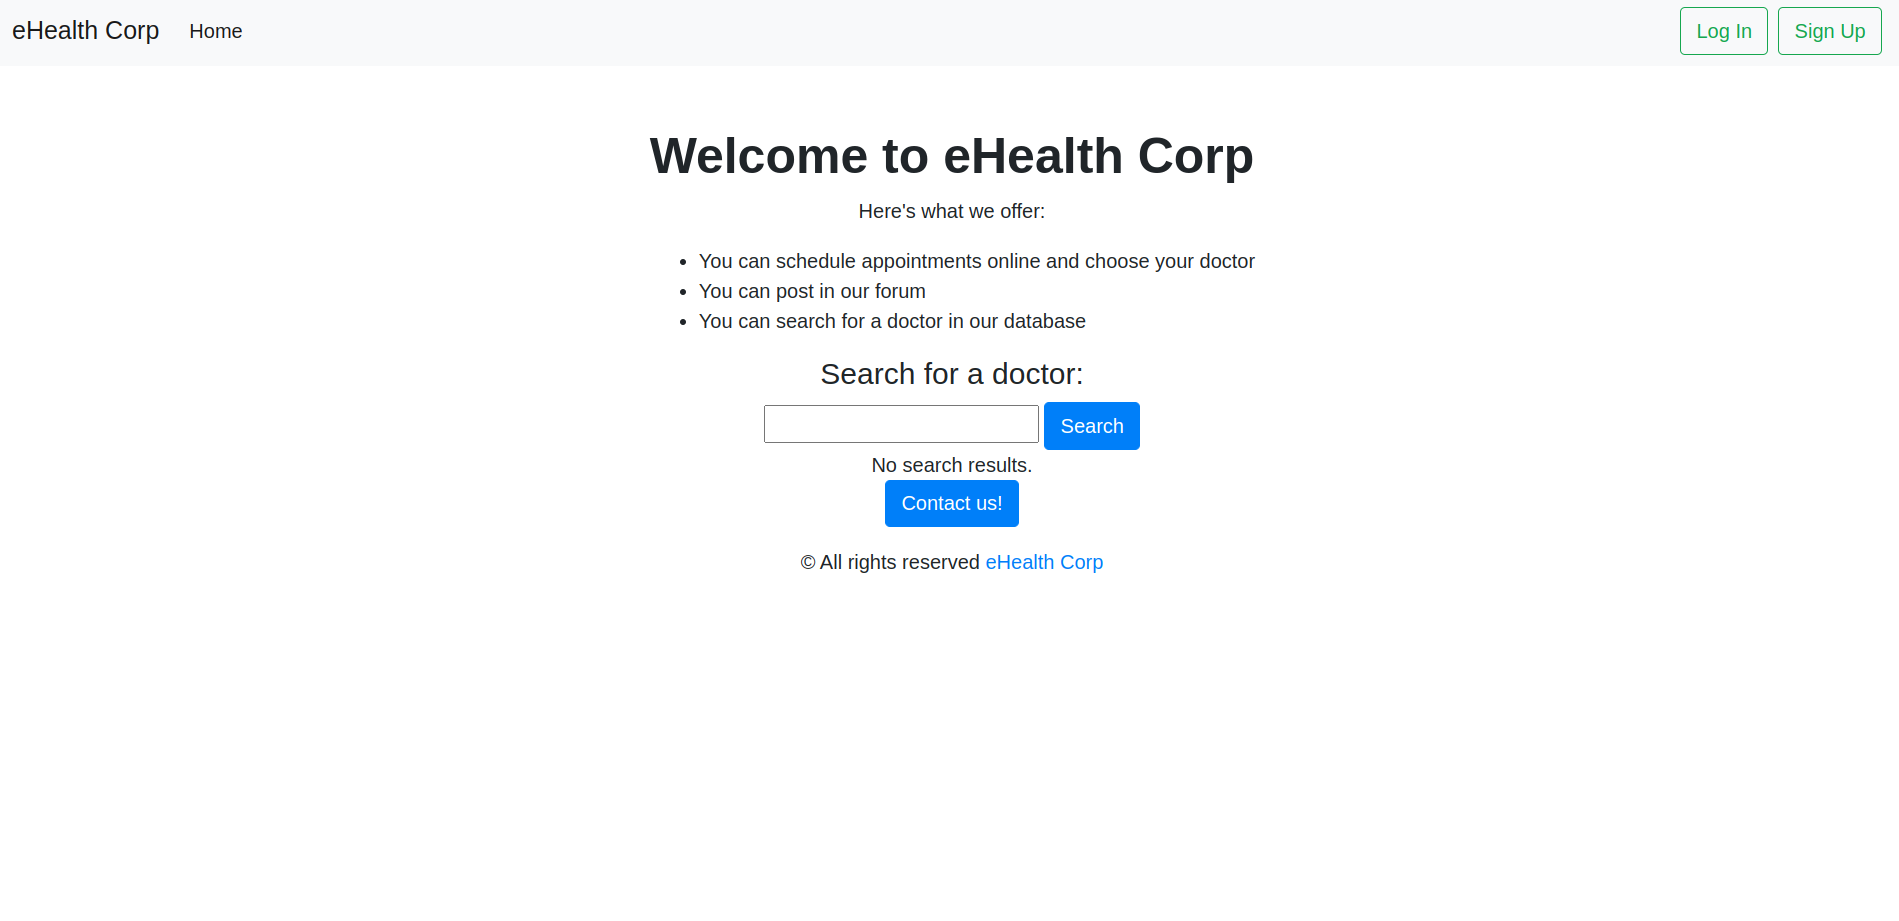
\includegraphics[trim={0 50mm 0 0},clip, scale = 0.25]{img/Site/Home.png}}
\caption{Home page}
}
}\end{figure}

\newpage
\section{Forum}
 \quad A página do forum é o local onde se podem encontrar todas as publicações feitas pelos utilizadores do site, nesta página também é possível fazer as suas próprias publicações.
\begin{figure}[H]{
{
\shadowbox{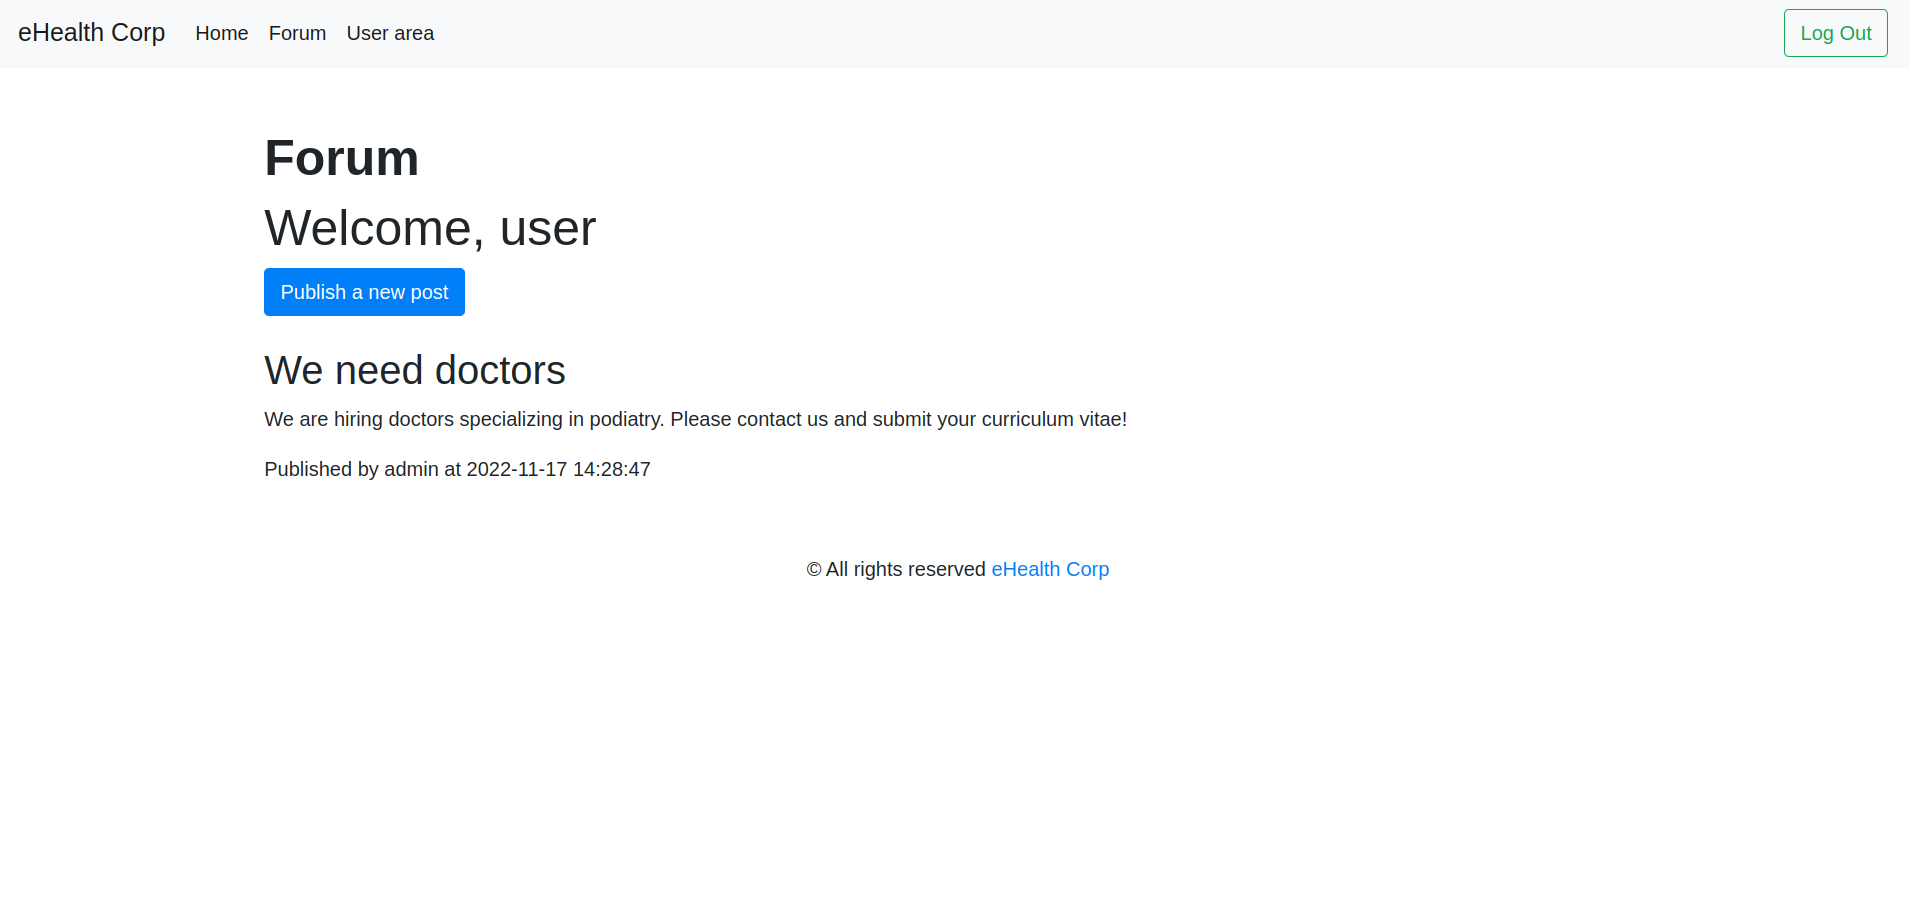
\includegraphics[trim={0 50mm 0 0},clip, scale = 0.25]{img/Site/Forum.png}}
\caption{Forum page}
}
}\end{figure}

\quad Para efetuar uma publicação pressiona se o botão de "Publish a new post" e para efetuar a publicação têm de se inserir os dados como o titulo e o contexto da publicação.
 
\begin{figure}[H]{
{
\shadowbox{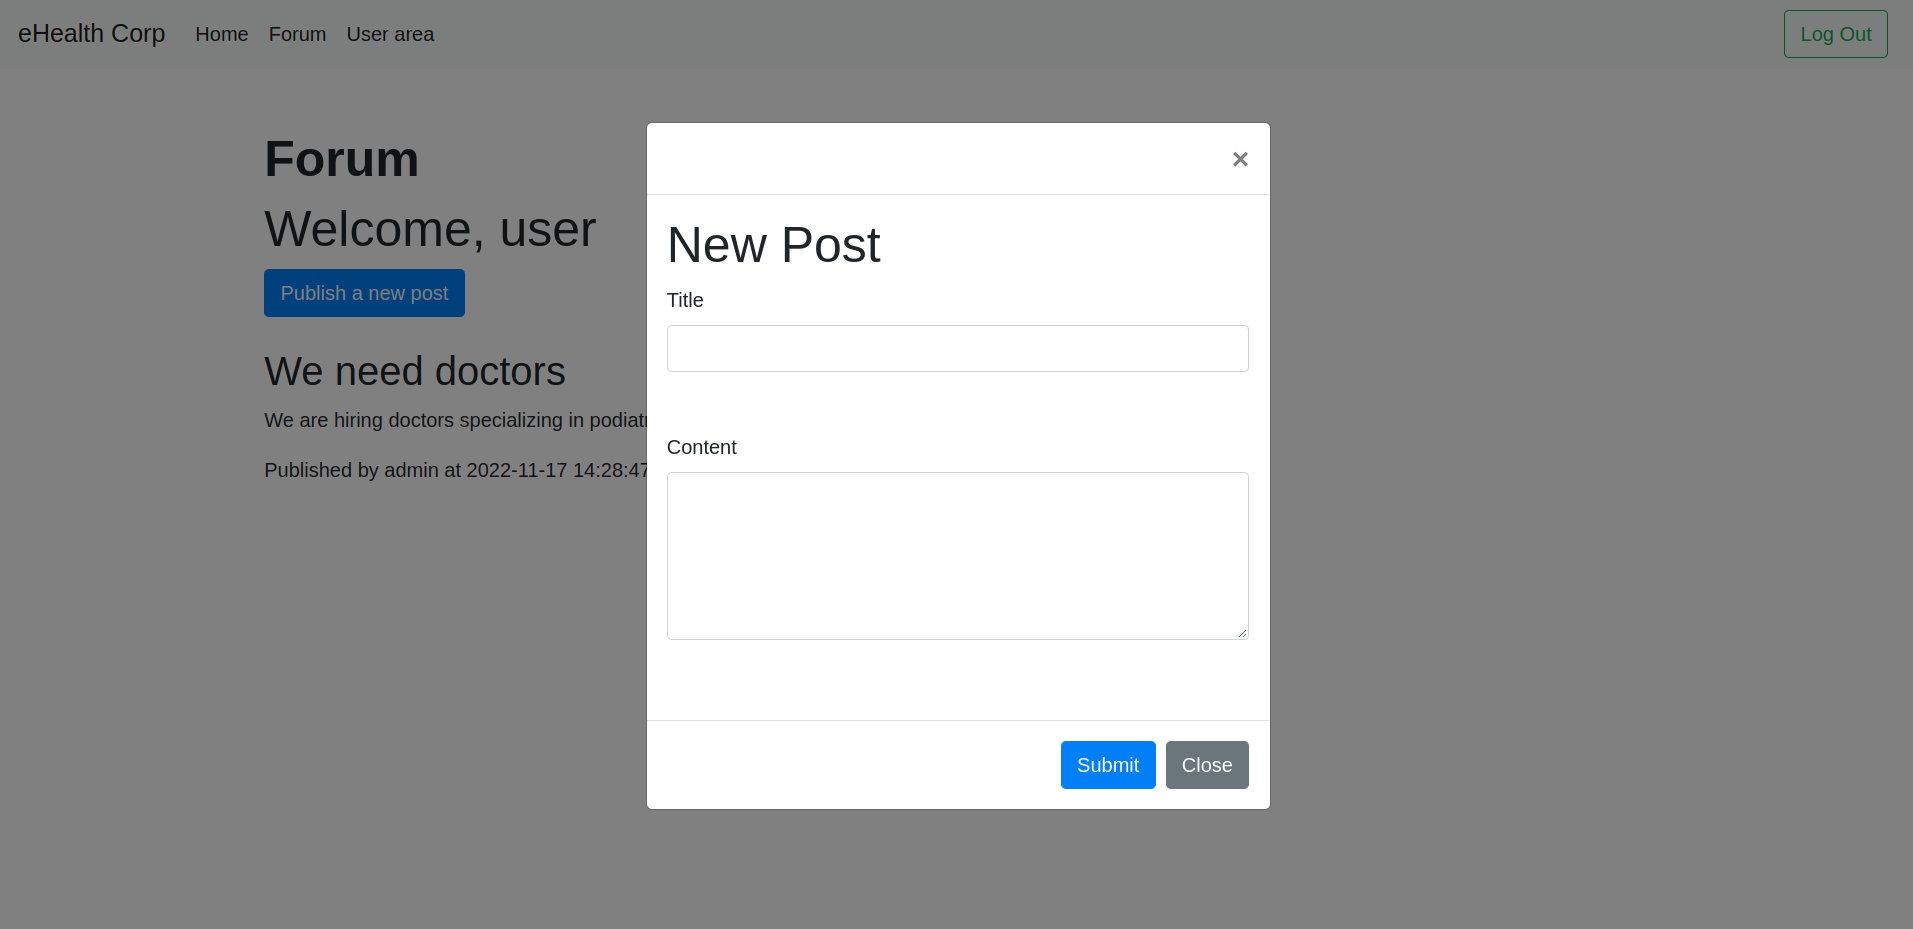
\includegraphics[trim={0 35mm 0 0},clip, scale = 0.25]{img/Site/NewPost.png}}
\caption{New Post Forum}
}
}\end{figure}

\newpage
\section{User Area}
\quad Na página da area do utilizador tem-se as informações do utilizador que está com o login efetuado, consegue-se observar informações como o user, a palavra-passe do user(encriptada), o seu nome completo e o seu email.\par
Nesta página também se encontram a lista de consultas que o utilizador tem marcado, a opção de as marcar caso seja desejado e por último a opção de guardar um certificado com todos os dados da consulta que foi inserido o id.
\newline
\begin{figure}[H]{
{
\shadowbox{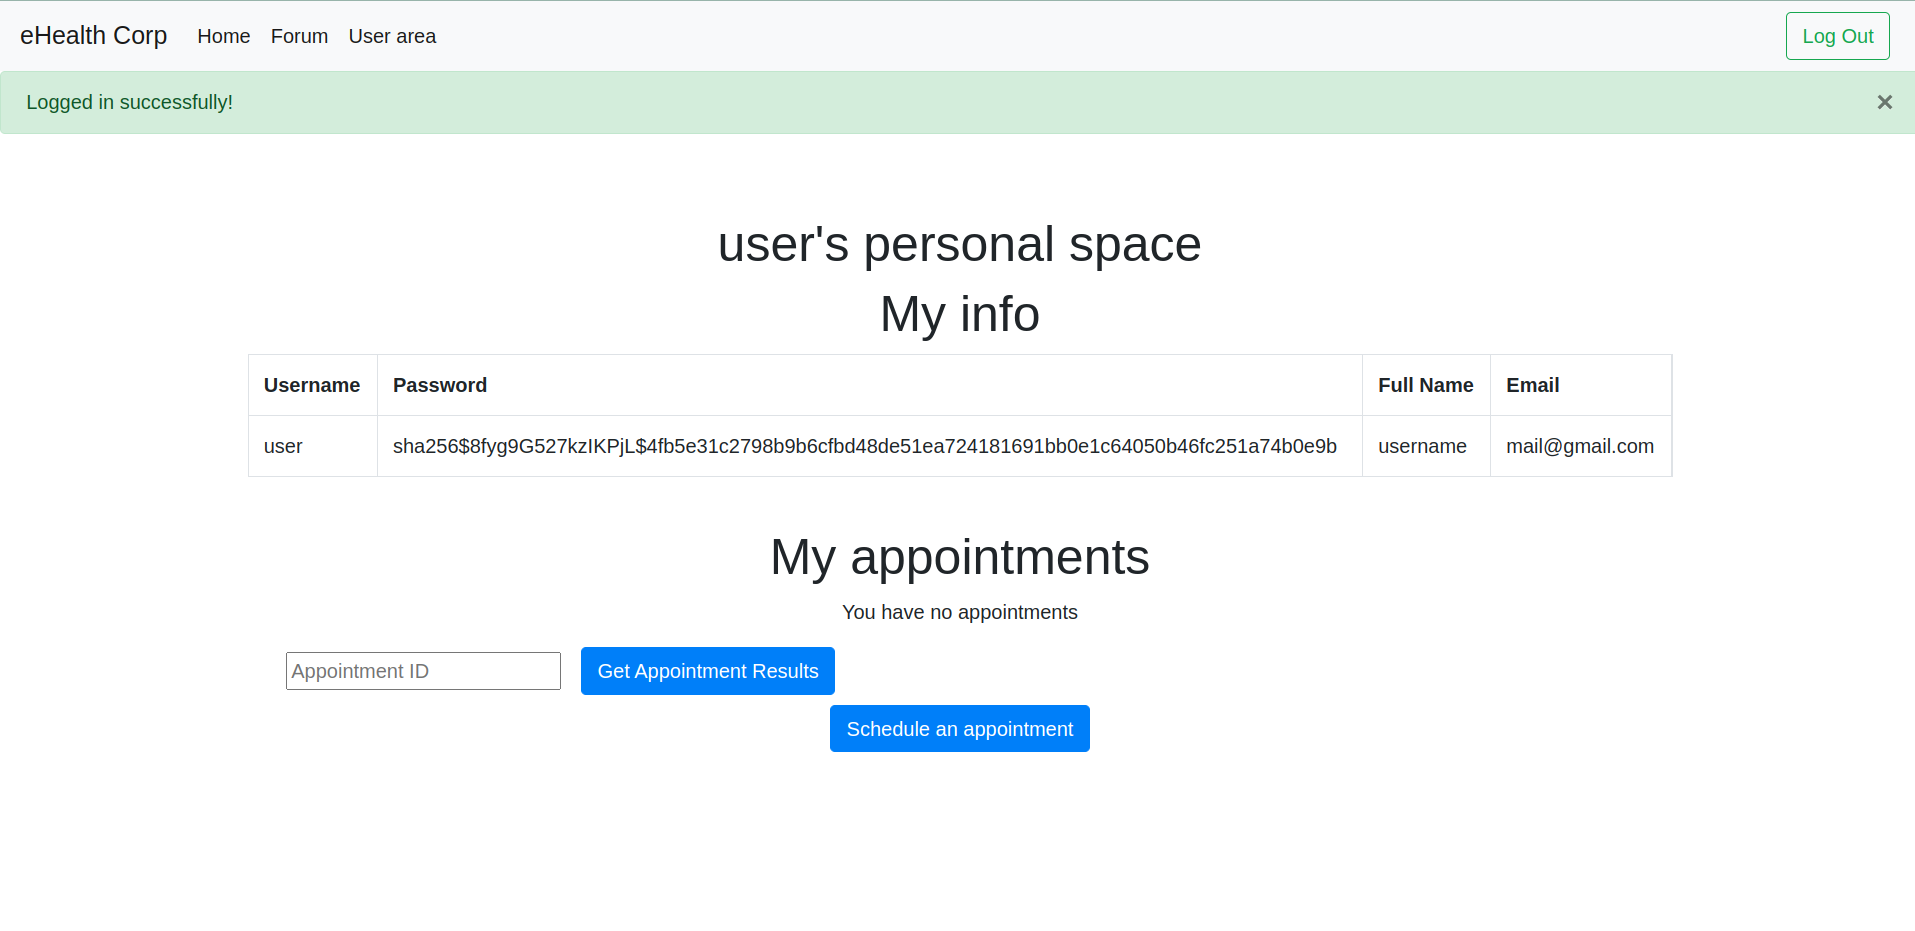
\includegraphics[trim={0 50mm 0 0},clip, scale = 0.25]{img/Site/UserArea.png}}
\caption{User area page}
}
}\end{figure}

\newpage
\section{Login}
\quad Ao se pressionar o botão de Login presente na home page é se redirecionado para a página de login, na qual se apresenta o local para inserir o utilizador e a sua palavra-passe para aceder à conta, caso esta já tenha sido previamente criada.
\begin{figure}[H]{
{
\shadowbox{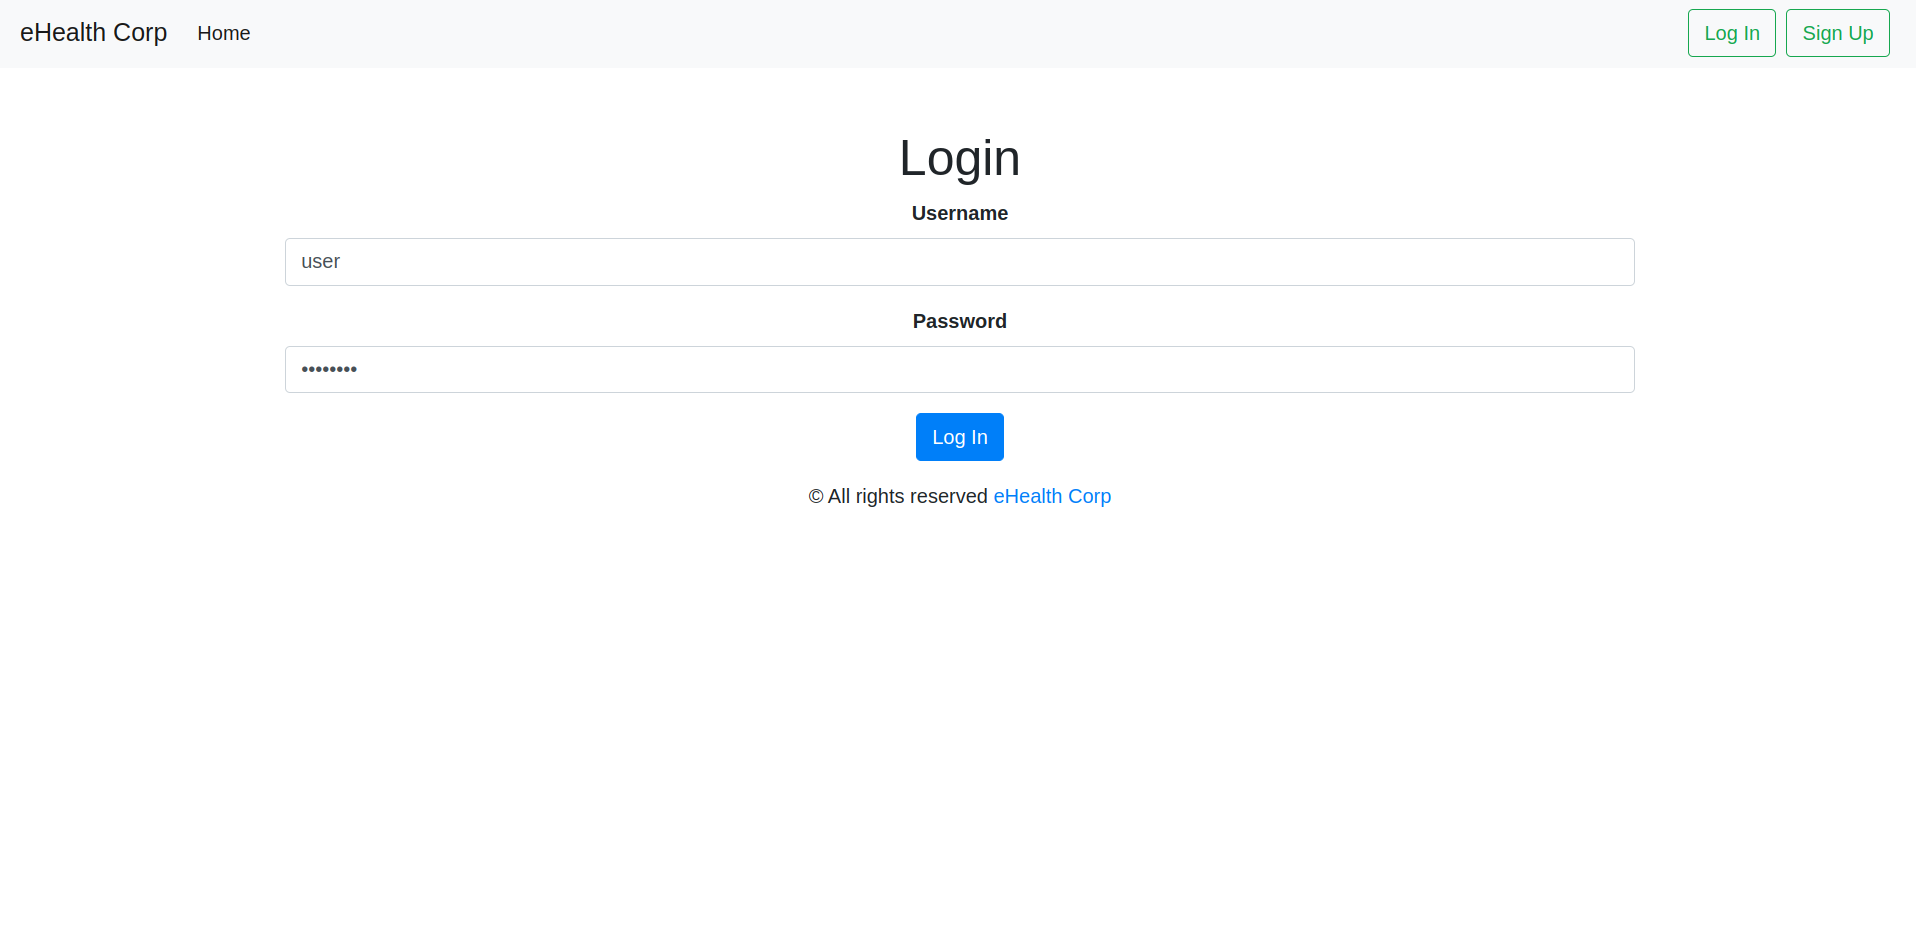
\includegraphics[trim={0 50mm 0 0},clip, scale = 0.25]{img/Site/LogIn.png}}
\caption{Login page}
}
}\end{figure}


\section{Sign up}
\quad Ao se pressionar o botão de Sign up na home page é se redirecionado para a página Sign up, esta serve para o utilizador criar uma conta, para isso têm de ser inseridos os seguintes dados: nome de utilizador,nome completo, mail, palavra-passe e a sua confirmação. Após isto, o utilizador poderá efetuar o login na página normalmente.
\begin{figure}[H]{
{
\shadowbox{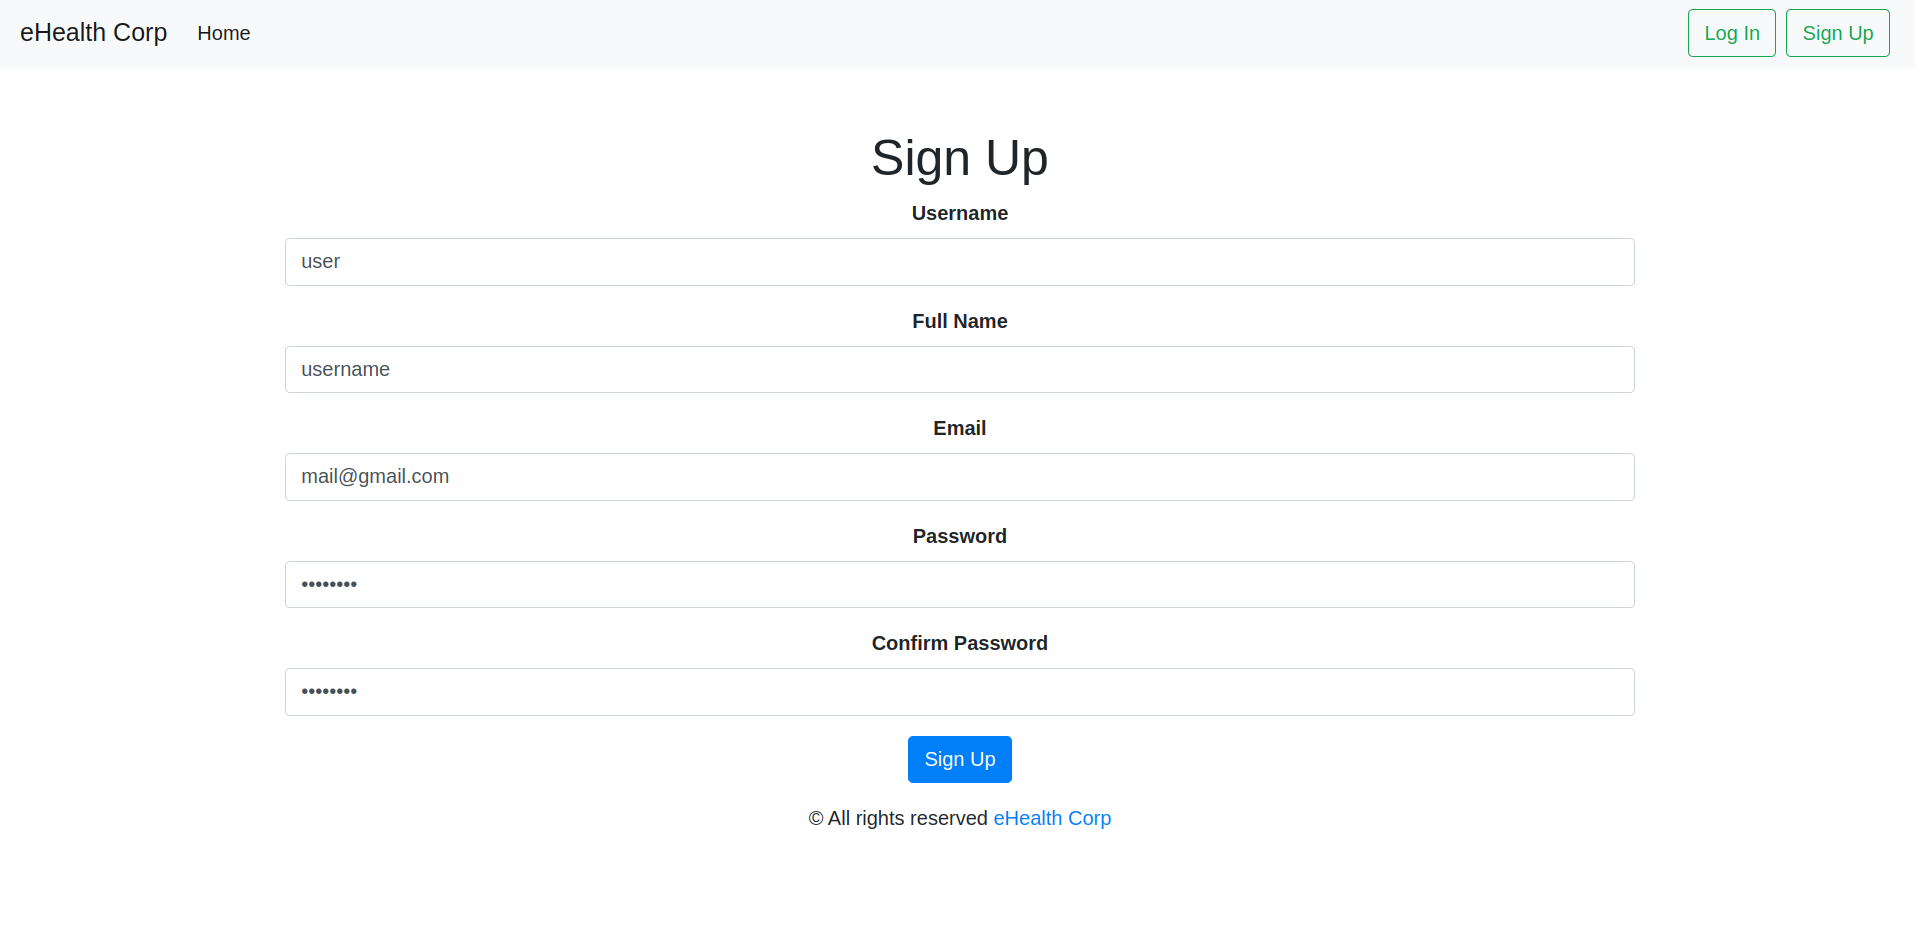
\includegraphics[trim={0 30mm 0 0},clip, scale = 0.25]{img/Site/SignUp.png}}
\caption{Sign up Page}
}
}\end{figure}

\chapter{Lista de Vulnerabilidades}\label{Vulnerabilidades}
\begin{itemize}
  \item[\ref{79}] CWE-79 - Cross-site Scripting
  \item[\ref{89}] CWE-89 - SQL Injection
  \item[\ref{284}] CWE-284 - Improper Access Control
  \item[\ref{200}] CWE-200 - Exposure of Sensitive Information to an Unauthorized Actor
  \item[\ref{521}] CWE-521 - Weak Password Requirements e CWE-20 - Improper Input Validation
  \item[\ref{425}] CWE-425 - Direct Request ('Forced Browsing')
  \item[\ref{256}] CWE-256 - Plaintext Storage of a Password
\end{itemize}

\newpage
\section{CWE-79 - Cross-site Scripting} \label{79}
A vulnerabilidade  CWE - 79, ou Cross Site Scripting, consiste em inserir scripts maliciosos em sites ou aplicações web. Isto ocorre devido ao facto do servidor não verificar a integridade dos inputs antes de os enviar ao cliente.\par

\begin{figure}[H]{
\centering
{
\shadowbox{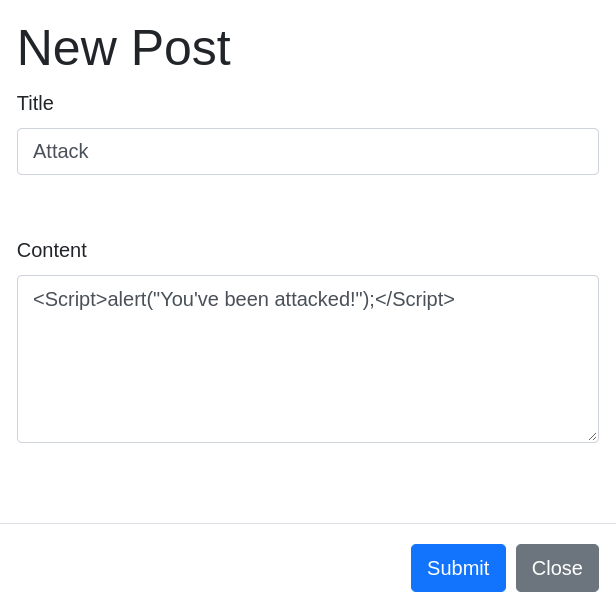
\includegraphics[trim={0 50mm 0 0},clip, scale = 0.5]{img/79/1-newpost.png}}
\caption{Criação de um script malicioso}
}
}\end{figure}


\begin{figure}[H]{
\centering
{
\shadowbox{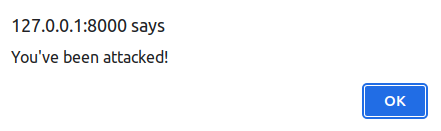
\includegraphics[trim={0 0 0 0},clip, scale = 0.75]{img/79/2-popup.png}}
\caption{Execução do script}
}
}\end{figure}

Na versão segura da app esta vulnerabilidade é corrigida através do uso do filtro \emph{safe} do flask/jinja2.

\begin{figure}[H]{
\centering
{
\shadowbox{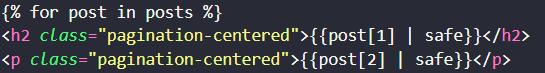
\includegraphics[trim={0 0 0 0},clip, scale = 0.75]{img/79/3-html.png}}
\caption{Versão segura}
}
}\end{figure}
A esta vulnerabilidade atribuímos o valor CVSS de 9.4. Para tal, considerámos o vetor de ataque network (pois os scripts podem ser executados através da rede), complexidade de ataque baixa (os scripts são relativamente simples), não requer privilégios por parte do atacante nem interação por parte de outro usuário para funcionar, não altera a scope (pois não afeta outras funcionalidades do servidor), existe alguma perda de confidencialidade, dependendo do script realizado pelo atacante, há uma alta perda de integridade e existe possibilidade do atacante bloquear completamente o acesso ao serviço.\par
CVSS score: \begin{itemize}
  \item Attack vector: Network
  \item Attack Complexity: Low
  \item Privileges Required: None
  \item User Interaction: None
  \item Scope: None
  \item Confidentiality: Low
  \item Integrity: High
  \item Availability: High
\end{itemize}

\newpage
\section{CWE-89 - SQL Injection} \label{89}
A vulnerabilidade CWE - 89, ou SQL Injection, consiste em inserir scripts maliciosos que irão ter acesso a bases de dados associadas aos campos de input onde foi inserido o script.

\begin{figure}[H]{
\centering
{
\shadowbox{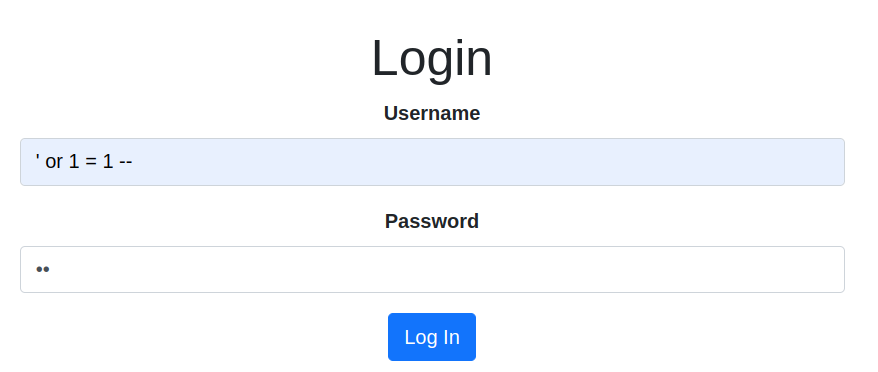
\includegraphics[trim={0 0 0 0},clip, scale = 0.5]{img/89 - 284/1-LoginSql.png}}
\caption{Criação do script}
}
}\end{figure}

\begin{figure}[H]{
\centering
{
\shadowbox{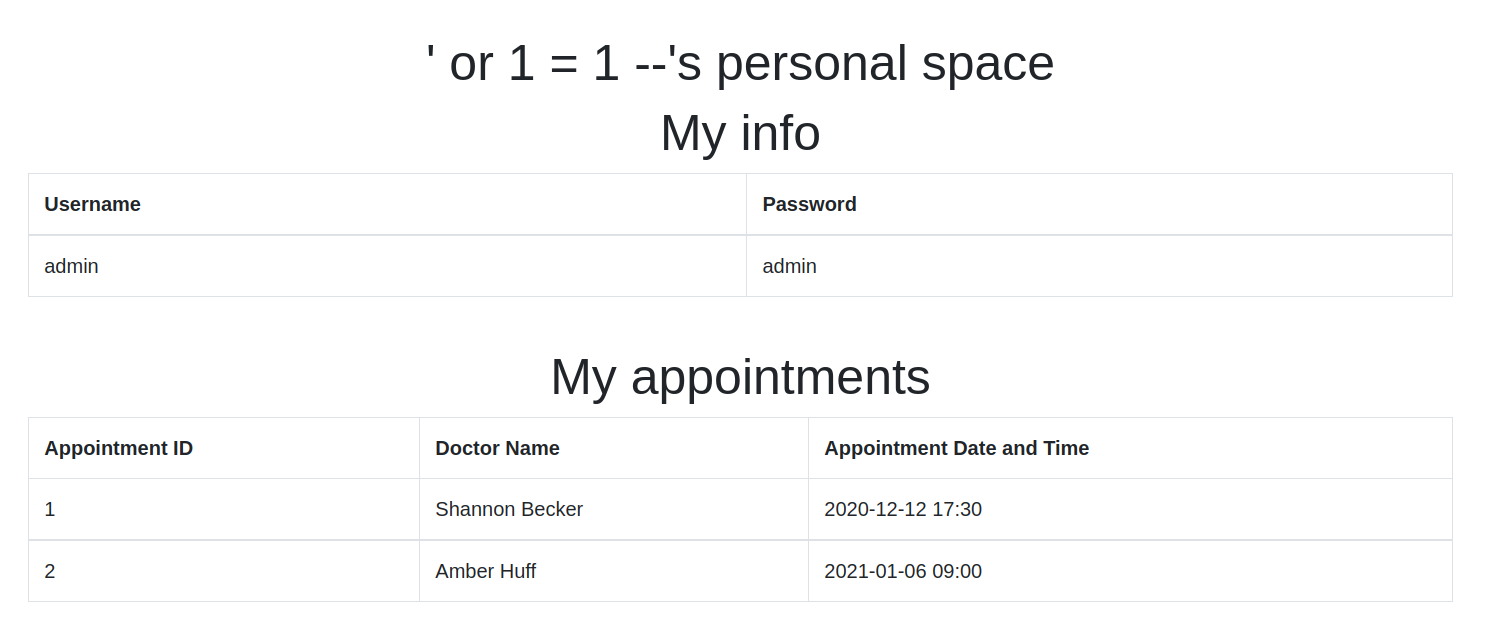
\includegraphics[trim={0 0 0 0},clip, scale = 0.3]{img/89 - 284/2-SqlPersonal.png}}
\caption{Execução do script}
}
}\end{figure}

Para solucionar este problema, tivemos de alterar a maneira como utilizávamos as bases de dados, passando a criá-las e utilizá-las de acordo com a API.


\begin{figure}[H]{
\centering
{
\shadowbox{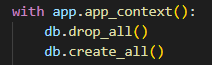
\includegraphics[trim={0 0 0 0},clip, scale = 2]{img/89 - 284/9-DBCreateright.png}}
\caption{Criação correta da base de dados}
}
}\end{figure}

\begin{figure}[H]{
\centering
{
\shadowbox{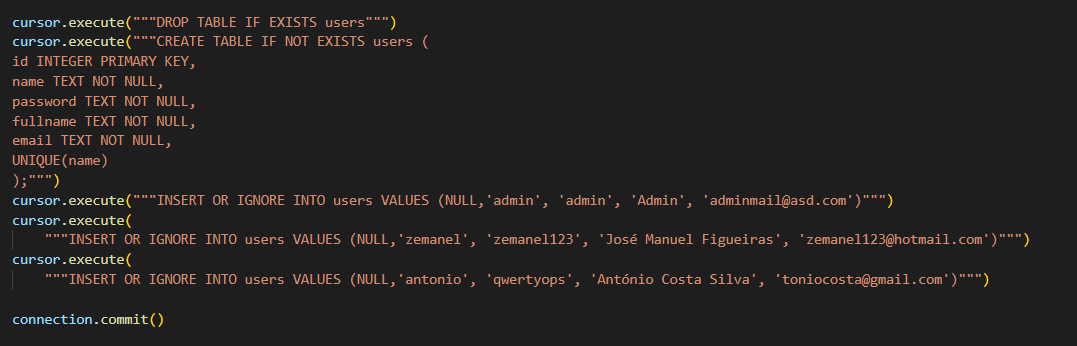
\includegraphics[trim={0 0 0 0},clip, scale = 0.75]{img/89 - 284/6-Wrongdb.png}}
\caption{Inserção de dados de maneira incorreta na base de dados}
}
}\end{figure}




\begin{figure}[H]{
\centering
{
\shadowbox{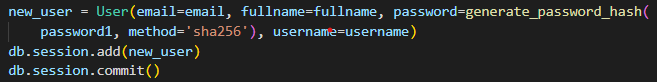
\includegraphics[trim={0 0 0 0},clip, scale = 1]{img/89 - 284/8-DBinsertright.png}}
\caption{Inserção de dados de maneira correta na base de dados}
}
}\end{figure}

\begin{figure}[H]{
\centering
{
\shadowbox{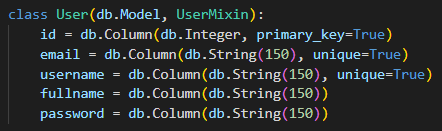
\includegraphics[trim={0 0 0 0},clip, scale = 1]{img/89 - 284/10-Usercreate.png}}
\caption{Criação da tabela de utilizadores da maneira correta}
}
}\end{figure}


Estes scripts podem ter vários efeitos, dependendo do código SQL injetado.\par

A esta vulnerabilidade atribuímos o valor CVSS de 9.8. Considerámos o vetor de ataque network, complexidade de ataque baixa (basta apenas um pouco de código SQL), não requer privilégios por parte do atacante nem interação por parte de outro usuário para funcionar, não altera a scope, existe uma alta perda de confidencialidade (pois o atacante irá ter acesso às credenciais de todos os utilizadores, há uma alta perda de integridade e existe possibilidade do atacante bloquear completamente o acesso ao serviço.\par
CVSS score: \begin{itemize}
  \item Attack vector: Network
  \item Attack Complexity: Low
  \item Privileges Required: None
  \item User Interaction: None
  \item Scope: None
  \item Confidentiality: High
  \item Integrity: High
  \item Availability: High
\end{itemize}

\newpage
\section{CWE-284 - Improper Access Control} \label{284}
Esta vulnerabilidade, de maneira semelhante à CWE - 89, pode ser explorada colocando o nome de um usuário já existente e colocando o script anterior no campo password, isto irá validar o login do usuário sem ser necessário obter a sua password.

\begin{figure}[H]{
\centering
{
\shadowbox{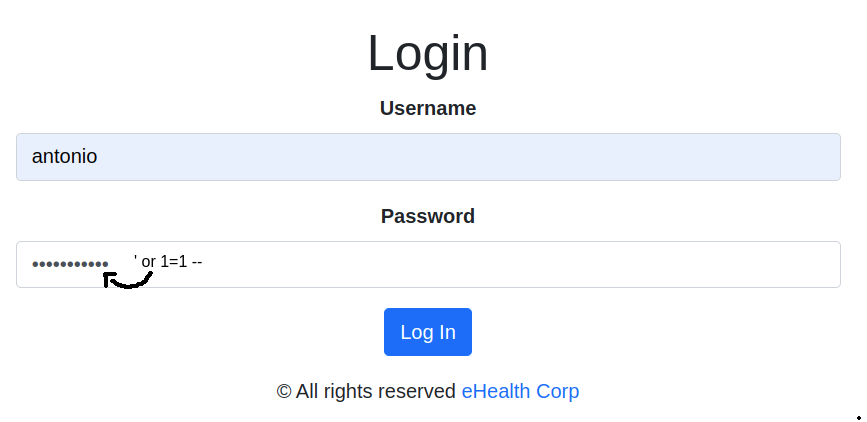
\includegraphics[trim={0 0 0 0},clip, scale = 0.5]{img/89 - 284/3-LoginSqlUser.png}}
\caption{Colocar o script no campo password}
}
}\end{figure}
\begin{figure}[H]{
\centering
{
\shadowbox{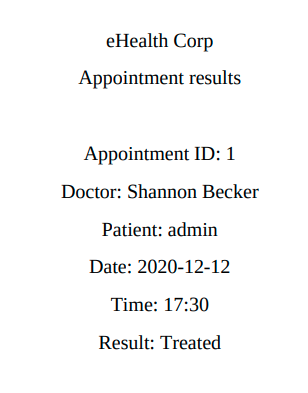
\includegraphics[trim={0 0 0 0},clip, scale = 0.5]{img/89 - 284/6-Certification.png}}
\caption{Acesso aos dados do utilizador}
}
}\end{figure}
\begin{figure}[H]{
\centering
{
\shadowbox{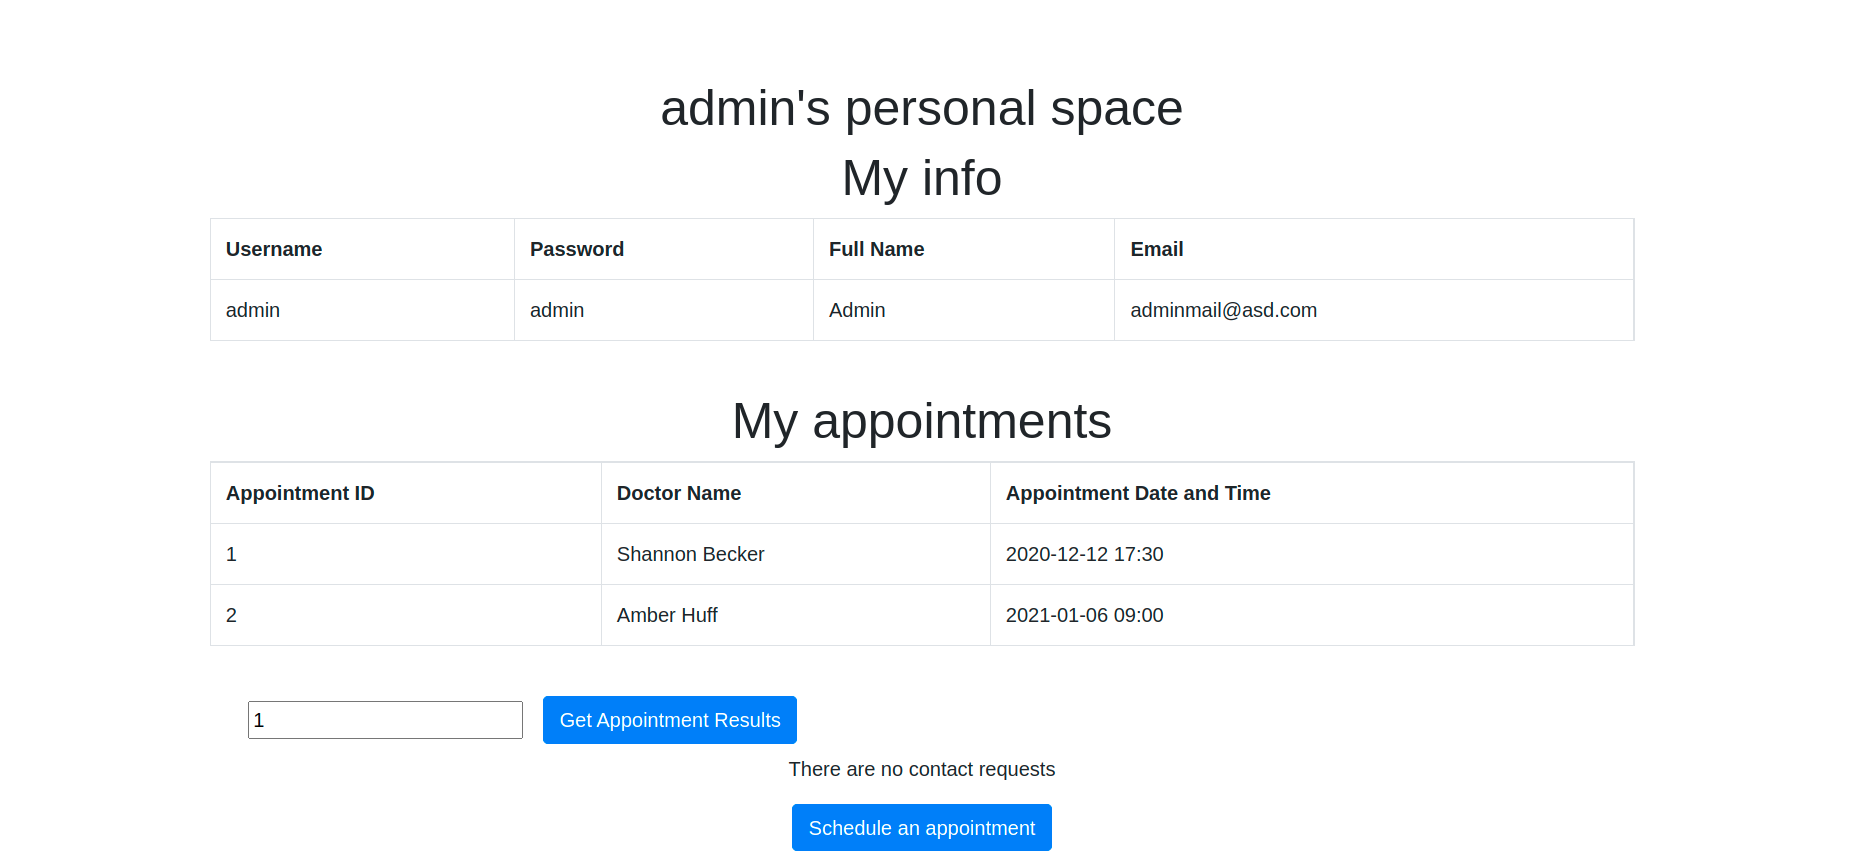
\includegraphics[trim={0 0 0 0},clip, scale = 0.25]{img/89 - 284/5-ProfileSql.png}}
\caption{Acesso à conta do utilizador}
}
}\end{figure}
A esta vulnerabilidade atribuímos o valor CVSS de 8.6. Considerámos o vetor de ataque network, complexidade de ataque baixa (basta apenas um pouco de código SQL), não requer privilégios por parte do atacante nem interação por parte de outro usuário para funcionar, não altera a scope, existe uma alta perda de confidencialidade (pois o atacante irá ter acesso à conta de qualquer utilizador), há alguma perda de integridade e o atacante pode cortar o acesso ao serviço apenas ao utilizador da conta comprometida (alterando a password).\par
CVSS score: \begin{itemize}
  \item Attack vector: Network
  \item Attack Complexity: Low
  \item Privileges Required: None
  \item User Interaction: None
  \item Scope: None
  \item Confidentiality: High
  \item Integrity: Low
  \item Availability: Low
\end{itemize}
\newpage
\section{CWE-200 - Exposure of Sensitive Information to an Unauthorized Actor} \label{200}
A vulnerabilidade CWE - 200 consiste na exposição de informação a utilizadores que não lhe deviam ter acesso. \par
No nosso caso, esta vulnerabilidade está evidente no url do site, onde qualquer utilizador pode alterar o url de modo a ter acesso a páginas de outros utilizadores.

\begin{figure}[H]{
\centering
{
\shadowbox{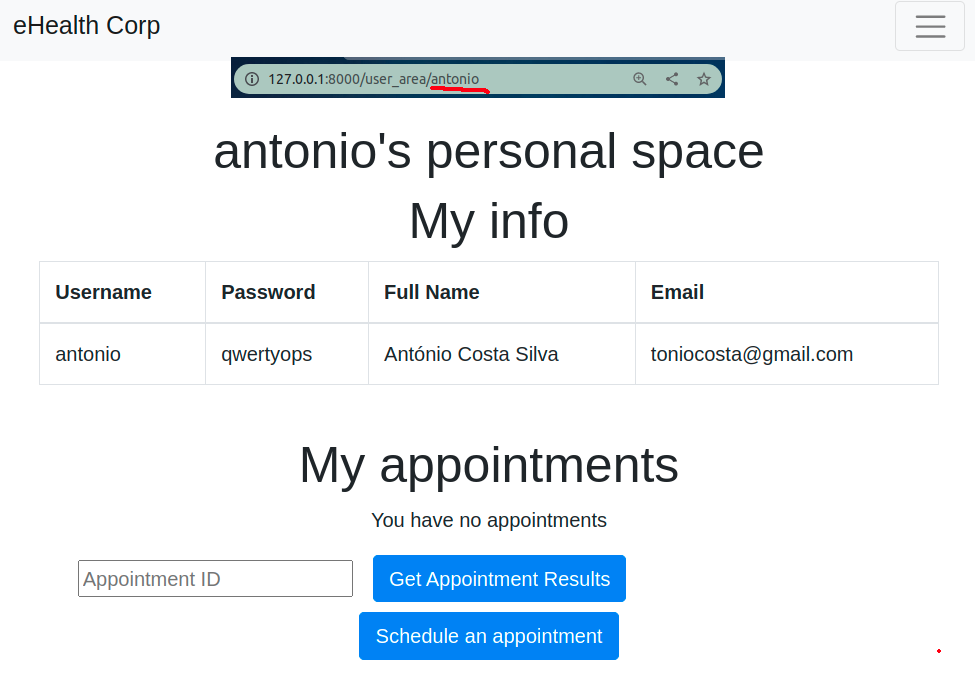
\includegraphics[trim={0 0 0 0},clip, scale = 0.4]{img/200/1-Profile.png}}
\caption{Acesso à página de um utilizador alterando o url}
}
}\end{figure}

Na versão segura do site esta vulnerabilidade foi corrigida ao utilizar a função \emph{login\_required} presente no flask. Esta função apenas vai permitir a visualização do conteúdo da página de um utilizador apenas se for esse utilizador que tenha feito login.

\begin{figure}[H]{
\centering
{
\shadowbox{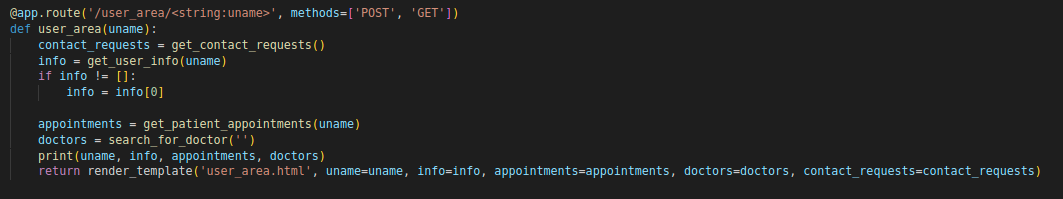
\includegraphics[trim={0 0 0 0},clip, scale = 0.4]{img/200/2-User.png}}
\caption{Versão insegura do código}
}
}\end{figure}

\begin{figure}[H]{
\centering
{
\shadowbox{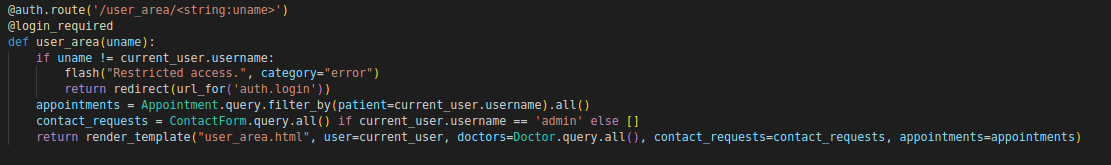
\includegraphics[trim={0 0 0 0},clip, scale = 0.4]{img/200/3-UserSec.png}}
\caption{Versão segura do código}
}
}\end{figure}
A esta vulnerabilidade atribuímos o valor CVSS de 8.6 pois os efeitos que esta causa no servidor irão ser muito semelhantes à vulnerabilidade CWE - 284, logo os seus parâmetros CVSS irão ser idênticos.\par
CVSS score: \begin{itemize}
  \item Attack vector: Network
  \item Attack Complexity: Low
  \item Privileges Required: None
  \item User Interaction: None
  \item Scope: None
  \item Confidentiality: High
  \item Integrity: Low
  \item Availability: Low
\end{itemize}

\newpage
\section{CWE-521 - Weak Password Requirements e CWE-20 - Improper Input Validation} \label{521}
As vulnerabilidades CWE - 521 e CWE - 20 são bastante semelhantes, por isso iremos analisá-las em conjunto. \par
A vulnerabilidade CWE - 521 consiste em não aplicar critérios rigorosos na criação da password de um utilizador, o que fará com que esta esteja mais vulnerável a ataques.\par
Para resolver este problema foram implementadas na versão segura da app uma série de medidas para aumentar a complexidade e segurança da password de um utilizador.\par

A vulnerabilidade CWE - 20 ocorre quando os dados introduzidos pelo utilizador não são devidamente tratados, o que pode levar a erros e conflitos, visto que muitos desses dados estarão presentes no url.\par
Para resolver esta vulnerabilidade foi criada a função \emph{replace\_all()} para substituir todos os carateres que poderiam gerar problemas por versões seguras dos mesmos.

\begin{figure}[H]{
\centering
{
\shadowbox{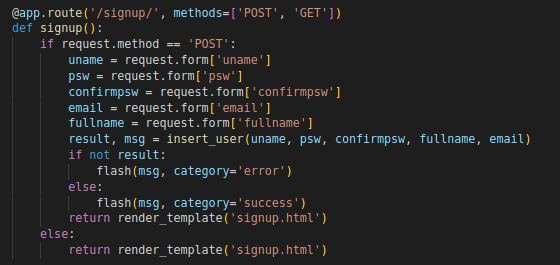
\includegraphics[trim={0 0 0 0},clip, scale = 0.75]{img/521 - 20/1-SignUp.png}}
\caption{Versão insegura do código}
}
}\end{figure}

\begin{figure}[H]{
\centering
{
\shadowbox{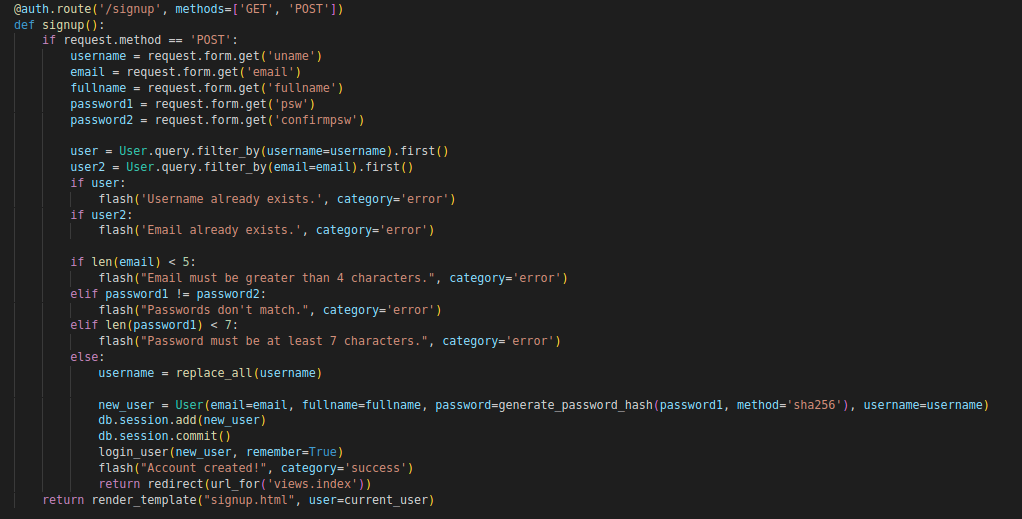
\includegraphics[trim={0 0 0 0},clip, scale = 0.5]{img/521 - 20/2-SignUpSec.png}}
\caption{Versão segura do código}
}
}\end{figure}
A estas vulnerabilidades atribuímos o valor CVSS de 7. Para tal, considerámos o vetor de ataque network, complexidade de ataque alta (pois o atacante ainda terá de investir em outro software para aceder às bases de dados), não requer privilégios por parte do atacante nem interação por parte de outro usuário para funcionar, não altera a scope, existe uma alta perda de confidencialidade (caso o atacante consiga aceder à conta de outro utilizador), ocorre alguma perda de integridade  e o atacante consegue cortar o acesso aos recursos do site apenas ao utilizador que atacou.\par
CVSS score: \begin{itemize}
  \item Attack vector: Network
  \item Attack Complexity: High
  \item Privileges Required: None
  \item User Interaction: None
  \item Scope: None
  \item Confidentiality: High
  \item Integrity: Low
  \item Availability: Low
\end{itemize}

\newpage
\section{CWE-425 - Direct Request ('Forced Browsing')} \label{425}
Esta vulnerabilidade ocorre quando o site ou aplicação não aplica restrições em url's, scripts ou ficheiros restritos, como páginas que iriam precisar de login para serem acessadas.\par

\begin{figure}[H]{
\centering
{
\shadowbox{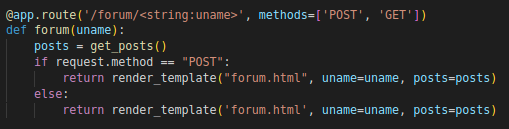
\includegraphics[trim={0 0 0 0},clip, scale = 1]{img/425/1-Force.png}}
\caption{Versão insegura do código}
}
}\end{figure}

Para resolver a vulnerabilidade foi adicionado um \emph{decorator} a páginas restritas para efetivamente verificar se foi efetuado o login e se o login foi efetuado pelo utilizador que está a tentar acessar a página.

\begin{figure}[H]{
\centering
{
\shadowbox{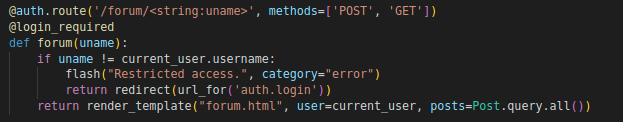
\includegraphics[trim={0 0 0 0},clip, scale = 0.75]{img/425/2-ForceSec.png}}
\caption{Versão segura do código}
}
}\end{figure}

\newpage
A esta vulnerabilidade atribuímos o valor CVSS de 5.3. Para tal, considerámos o vetor de ataque network, complexidade de ataque baixa, não requer privilégios por parte do atacante nem interação por parte de outro usuário para funcionar, não altera a scope, existe alguma perda de confidencialidade (uma vez que o atacante irá ter acesso a conteúdos restritos), não ocorre qualquer perda de integridade nem qualquer perda de acesso aos serviços.\par
CVSS score: \begin{itemize}
  \item Attack vector: Network
  \item Attack Complexity: Low
  \item Privileges Required: None
  \item User Interaction: None
  \item Scope: None
  \item Confidentiality: Low
  \item Integrity: None
  \item Availability: None
\end{itemize}
\newpage

\section{CWE-256 - Plaintext Storage of a Password} \label{256}
Esta vulnerabilidade ocorre quando as passwords criadas pelos utilizadores são guardadas numa base de dados em plain text, ou seja, texto não encriptado. Com isto surgem vários problemas caso uma base de dados seja vítima de um ataque, pois o atacante terá acesso a todas as passwords imediatamente.

\begin{figure}[H]{
\centering
{
\shadowbox{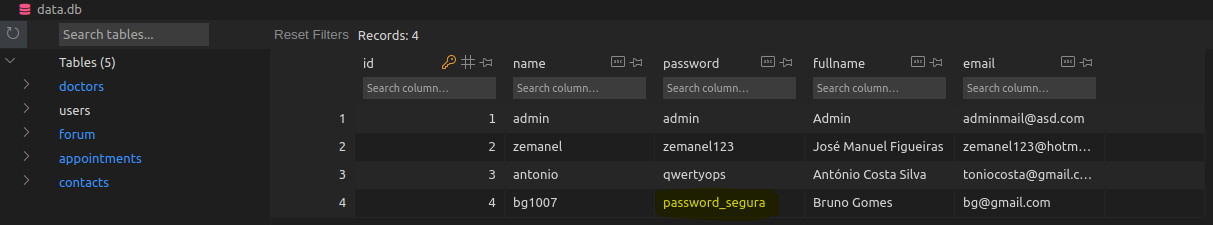
\includegraphics[trim={0 0 0 0},clip, scale = 0.7]{img/256/db_unsafe.PNG}}
\caption{Passwords em plain text na base de dados insegura}
}
}\end{figure}

\begin{figure}[H]{
\centering
{
\shadowbox{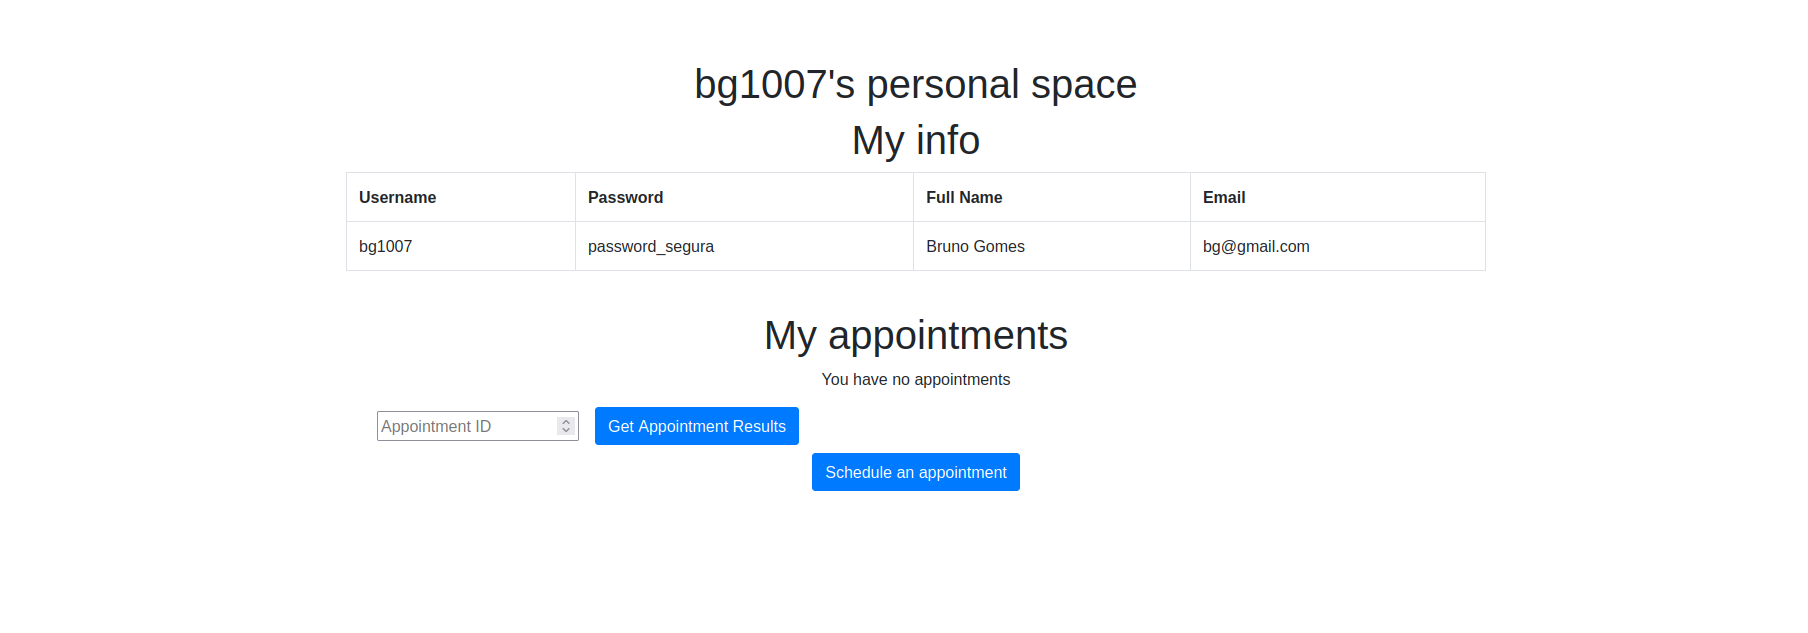
\includegraphics[trim={0 0 0 0},clip, scale = 0.45]{img/256/password_sem_seguranca.PNG}}
\caption{Display da password}
}
}\end{figure}

Como podemos ver no código abaixo, a password é guardada em texto normal, sem qualquer tipo de encriptação

\begin{figure}[H]{
\centering
{
\shadowbox{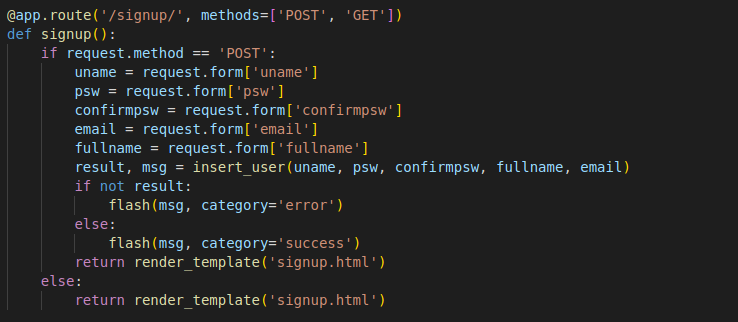
\includegraphics[trim={0 0 0 0},clip, scale = 1]{img/256/sign_up_sem_seguranca.PNG}}
\caption{Versão não segura do código}
}
}\end{figure}

Para resolver a vulnerabilidade, as passwords foram encriptadas utilizando o algoritmo SHA-256, para que as passwords não pudessem ser lidas diretamente.

\begin{figure}[H]{
\centering
{
\shadowbox{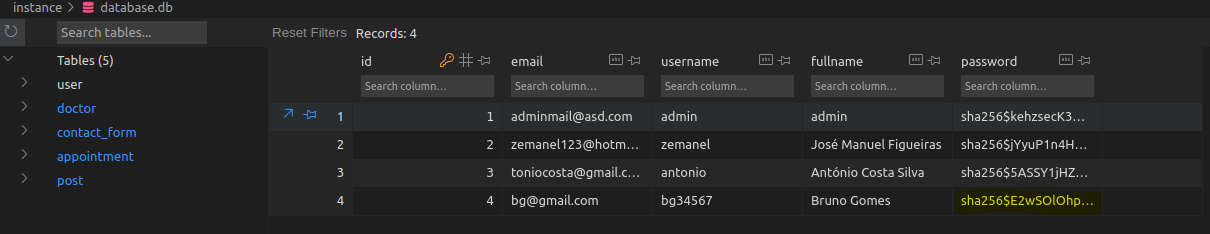
\includegraphics[trim={0 0 0 0},clip, scale = 0.7]{img/256/db_safe.PNG}}
\caption{Passwords encriptadas na base de dados segura}
}
}\end{figure}

\begin{figure}[H]{
\centering
{
\shadowbox{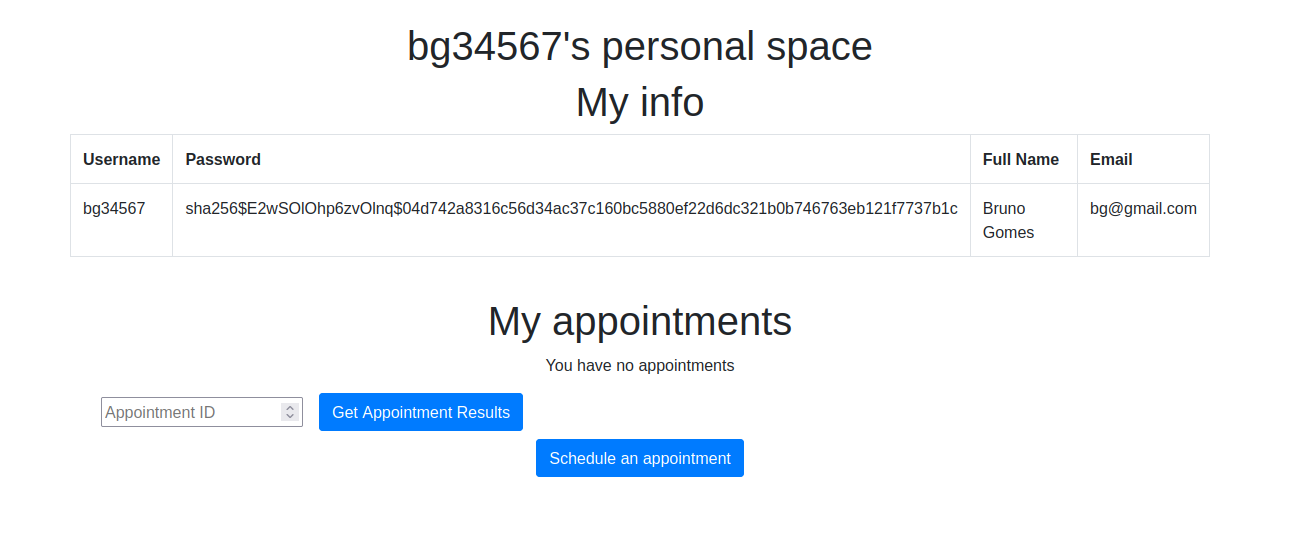
\includegraphics[trim={0 0 0 0},clip, scale = 0.5]{img/256/password_segura.PNG}}
\caption{Display da password}
}
}\end{figure}

\begin{figure}[H]{
\centering
{
\shadowbox{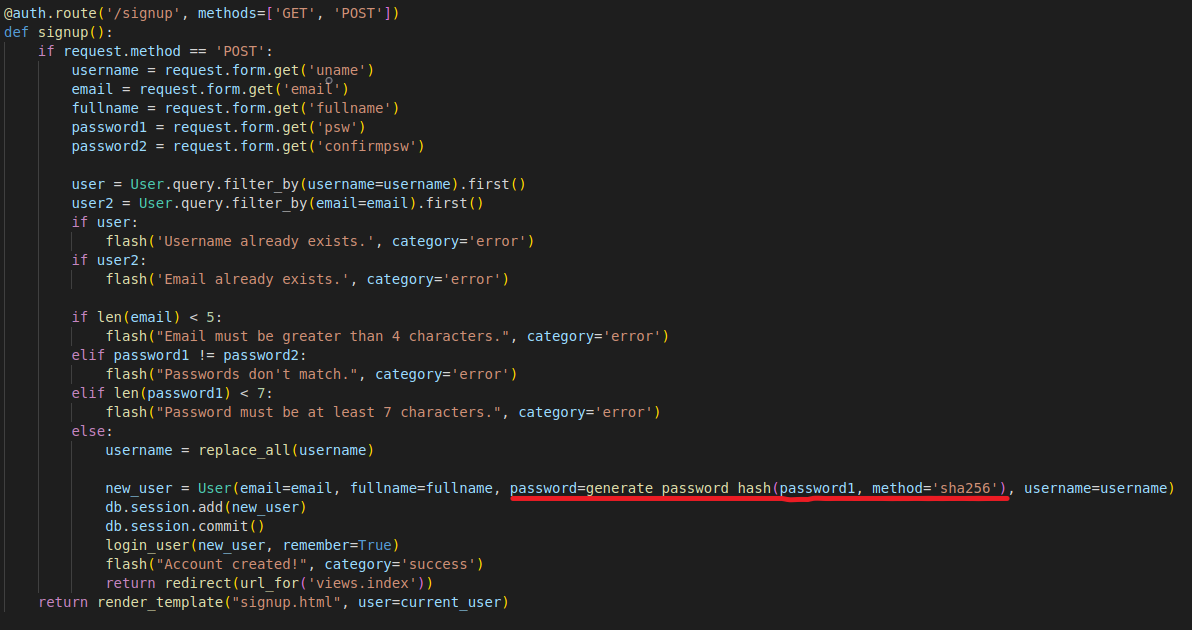
\includegraphics[trim={0 0 0 0},clip, scale = 0.5]{img/256/sign_up_seguro.PNG}}
\caption{Versão segura do código}
}
}\end{figure}

A esta vulnerabilidade atribuímos o valor CVSS de 7. Considerámos o vetor de ataque network, complexidade de ataque alta (pois o atacante ainda terá de investir em outro software para aceder às bases de dados), não requer privilégios por parte do atacante nem interação por parte de outro usuário para funcionar, não altera a scope, existe uma alta perda de confidencialidade (caso o atacante consiga aceder à conta de outro utilizador), ocorre alguma perda de integridade  e o atacante consegue cortar o acesso aos recursos do site apenas ao utilizador que atacou.\par 
CVSS score: \begin{itemize}
  \item Attack vector: Network
  \item Attack Complexity: High
  \item Privileges Required: None
  \item User Interaction: None
  \item Scope: None
  \item Confidentiality: High
  \item Integrity: Low
  \item Availability: Low
\end{itemize}

\newpage

\chapter{Conclusão}
  \quad Ao longo da realização deste projeto, viemos a descobrir muitos dos mecanismos que permitem o funcionamento dos sites e aplicações web que usamos tão frequentemente. Viemos também a descobrir muitas das falhas e vulnerabilidades existentes nestes serviços, pois embora o projeto fosse focado em tais vulnerabilidades, enquanto implementávamos uma, surgiam outras pelas quais não esperávamos, o que nos deu a conhecer um pouco do processo de desenvolvimento deste tipo de serviços.\par
  Ao corrigirmos as vulnerabilidades implementadas e corrigindo outras das quais não estávamos à espera, acabámos o projeto com um score cvss de 55.7, bastante superior ao esperado, mas que mesmo assim conseguimos corrigir por completo.
  
  \newpage



\chapter{Contribuidores}
O Trabalho foi analisado, discutido e realizado por
\begin{itemize}
  \item Bruno Gomes 103320
  \item João Gonçalves 98287
  \item João Oliveira 102631
  \item Marco Almeida 103440
\end{itemize}

\end{document}
